\section{Dynamical Berry's phase and non-linear response} 
\label{chapterberry}
\subsection{Why do we need Berry's phase?}
%In this work we use dynamical Berry's phase to calculate the non-linear response in extended systems. 
%This section presents a simple introduction to the problem of polarisation definition in extended systems and how it can be solved by means of Berry's phase concept.
%\begin{wrapfigure}{r}{0.5\textwidth}
%  \begin{center}
%    
\includegraphics[width=0.4\textwidth]{Figures/wrong_polarization2}
%  \end{center}
%  \caption{Surface contribution to the polarisation in a solid. \label{surfacepol}}
%\end{wrapfigure}
For many years an unsolved problem in solid state physics was the correct definition of polarisation in periodic systems.
This definition is intrinsically related to the one the dipole operator, that is a problematic object for extended systems.
In the literature different wrong definitions of bulk polarisation have been proposed that we will not cite here\cite{restanotes}.
%In order to understand the problem, let's start the discussion from the polarisation in isolated systems.
%In a system with open boundary conditions, the dipole operator is well defined and therefore one can write down the polarisation as:
%\be
%\PP = \frac{e \langle \vec \rr \rangle}{V} = \frac{e}{V}\int \vec \rr n (\rr) d \rr,
\label{polisolated}
%%\ee
%where $n(\rr)$ is the electronic density.
%The simplest idea for the definition of the polarization in periodic systems would be to generalise the previous formula. The integral in Eq.~\ref{polisolated} can be redefined in different possible ways in periodic systems. We can average the dipole operator on the whole material or consider its unit cell. In the first case we obtain $ \PP = \langle \vec \rr \rangle_{sample}/V_{sample}$. In an insulator the contributions from the dipoles inside the material cancel each other (as one can see from  Fig.~\ref{immerse}) and only the surfaces contribute to the total polarisation (see Fig.~\ref{surfacepol}):                              
%\be
%\Delta \PP = \frac{(\Delta \sigma L^2) L }{L ^3},
%\label{polsurface}
%\ee
%where $\Delta \sigma$ is related to the charges accumulated on the surfaces.\cite{vanderbilt1993electric} 
%This definition [Eq.~\ref{polsurface}] is not suitable for numerical calculations because it requires the simulation of the entire sample and moreover the above defined polarisation is not a bulk property but it depends from the surfaces.\\ 
%The second possibility is to define the polarisation as  $ \PP = \langle \vec \rr \rangle_{cell}/V_{cell}$. But this definition is completely arbitrary. In fact different choices of the unit cell give completely different polarisations for the same material, see Fig.~\ref{cellpol}. A last possibility exists, the use of the dipole matrix elements in terms of Bloch orbitals, but also in this case there is problem since the dipole operator is unbounded in periodic systems.\\
%\begin{wrapfigure}{l}{0.5\textwidth}
%    \vspace{-0.7cm}
%%  \begin{center}
%    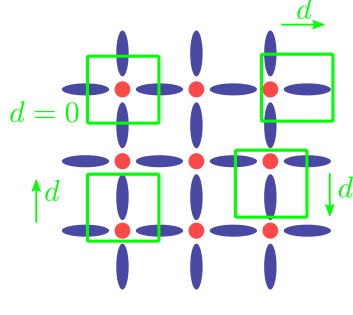
\includegraphics[width=0.4\textwidth]{Figures/wrong_polarization1}
%%%  \end{center}
%  \caption{Polarisation vector versus the choice of the unit cell. \label{cellpol} }
%\end{wrapfigure}
%Finally let mention that also the well know Clausius-Mossotti formula for the polarisability\cite{Mossotti} cannot be used in real solids because wave-functions are not localised objects.\\
Two reasons make polarisation definition so difficult in solids. First the dipole operator is ill defined in periodic systems, because $\vec \rr$ is not periodic while wave-functions are. Second, differently from finite systems, the polarisation cannot be expressed as an integral on the charge density\cite{Martin1998}.
This second aspect can be better understood if we write down the general relation between polarisation and density:
\be
\nabla \cdot \PP(\rr) = - n(\rr).
\ee                              
In finite systems we impose the condition  $\PP(\rr) \rightarrow 0 $ outside the sample (Dirichlet boundary condition) and $\int n(\rr) d\rr=0$.
In periodic system, it is most useful to resolve the previous equation into Fourier components $\qq+ \GG$,
where $\GG$ denotes a reciprocal lattice vector and $\qq$ belongs to the first Brillouin zone(BZ):
\be
(\qq + \GG) \cdot \PP(\qq + \GG) = i n (\qq + \GG).
\label{poldens}
\ee
It follows from Eq.~\ref{poldens} that each Fourier component can be treated separately. Now let us consider the limit $\GG=0$ and $\qq \rightarrow 0$. In this limit  the macroscopic polarisation $\PP$ is not determined anymore by the zero Fourier component of the density, which must vanish by charge neutrality.  Thus in the limit $\qq = 0$ for an infinite crystal, the polarisation contains additional information not included in the density.\cite{Martin1998} \\
The problem of a correct definition of polarisation in periodic systems was solved in 1993 by  King-Smith and Vanderbilt.\cite{KSV1} In their seminal paper they shown that  bulk polarisation can be expressed as a closed integral on the wave-function phase in the Brillouin zone, a particular case of the Berry's phase. Their formulation solved all problems with the previous attempts to define the polarisation. In fact the King-Smith and Vanderbilt(KSV) polarisation is a bulk quantity, its time derivative gives the current and its derivatives respect to the external field reproduce the polarisabilities at all orders.\\
\subsection{Response functions and bulk polarization}
\emph{Ab-initio} approaches based on Green's function theory became a standard tool for quantitative and predictive calculations of linear response optical properties in Condensed Matter. In particular, the state-of-the-art approach combines the $G_0W_0$ approximation for the quasi-particle band structure~\cite{aryasetiawan1998gw} with the Bethe-Salpeter equation in static ladder approximation for the response function.~\cite{strinati} This approach proved to effectively and accurately account for the essential effects beyond independent particle approximation (IPA) in a wide range of electronic systems, including extended systems with strong excitonic effects.~\cite{Onida}

In contrast, for nonlinear optics \ai calculations of extended systems rely in large part on the IPA\cite{PhysRevB.48.11705} with correlation effects entering at most as a rigid shift of the conduction energy levels\cite{PhysRevB.80.155205}.  Within time-dependent density-functional theory (TDDFT), it has been recently proposed~\cite{PhysRevB.82.235201} an approach to calculate the second-harmonic generation (SHG) in semiconductors that takes into account as well crystal local-field and excitonic effects. However, this promising approach~\cite{Cazzanelli2012} is limited by the treatment of the electron correlation to systems with weakly bound excitons.~\cite{LRC} 

%In fact, it is extremely involved to include many-body effects into the expression for the nonlinear optical susceptibilities within Green's function theory. 
%In fact, the inclusion of many-body effects in the equations for the non-linear susceptibilities makes them very difficult to solve.
Within Green's function theory the inclusion of many-body effects into the expression for the nonlinear optical susceptibilities is extremely difficult. 
Furthermore the complexity of these expressions grows with the perturbation order. Therefore it is not surprising that there have been only few isolated attempts to calculate second-order optical susceptibility using the Bethe-Salpeter equation~\cite{Leitsmann2005,Chang2002} and no attempt to calculate higher-order optical susceptibilities.~\cite{PhysRevB.80.165318} 
%The complexity growing with the perturbation order, there have been only few isolated attempts at calculating second-order optical susceptibility using the Bethe-Salpeter equation,~\cite{Leitsmann2005,Chang2002} and in practice third-order optical susceptibility is untreatable.~\cite{PhysRevB.80.165318} 
%On the other hand, the origin of this limitation is the attempting to calculate the nonlinear optical susceptibility directly in terms of the electronic structure. 

Alternatively to the frequency-domain response-based approach, one can obtain the nonlinear optical susceptibility in time-domain from the dynamical polarisation $\PP$ of the system by using the expansion of $\PP$ in power of the applied field
\be
\label{eq:peopbf}
\PP= \chi^{(1)} \efield + \chi^{(2)} \efield^2 + \chi^{(3)} \efield^3 + \dots 
\ee 
This strategy is followed in several real-time implementations of TD-DFT\cite{PhysRevB.54.4484}. In these approaches the dynamical polarisation is obtained by numerical integration of the equations of motion (EOMs) for the Kohn-Sham system.\cite{takimoto:154114,castro:3425,meng:054110} So far applications regard mostly nonlinear optical properties in molecules.  

 
The time-domain approach presents three major advantages with respect to frequency-domain response-based approaches. First, many-body effects are included easily by adding the corresponding operator to the effective Hamiltonian. Second, it is not perturbative in the external fields and therefore it treats optical susceptibilities at any order without increasing the computational cost and with the only limitation dictated by the machine precision. Third, several non-linear phenomena and thus spectroscopic techniques are described by the same EOMs. For instance, by the superposition of several laser fields one can simulate sum- and difference-frequency harmonic generation, or four-waves mixing.\cite{boyd}

%In a recent work,~\cite{attaccalite} we proposed a real-time implementation of the Bethe-Salpeter equation, based on nonequilibrium Green's function formalism.
Although this approach shows very promising results for molecular systems, its extention to periodic system remains still limited.
In fact, due to the problems in defining the position operator and thus $\PP$, it is not trivial to apply Eq.~\eqref{eq:peopbf} to systems in which periodic boundary conditions (PBC) are imposed. As it was recognised for example in Ref.~\cite{PhysRevB.52.14636}, the same problem appears in the direct evaluation of the nonlinear optical susceptibility in frequency-response based approaches. In particular the dipole matrix elements between the periodic part of the Bloch functions are ill-defined when using the standard definition of the  position operator. In that case, it is possible to obtain correct expressions for the dipole matrix elements from perturbation theory~\cite{PhysRevB.52.14636,PhysRevB.48.11705,PhysRevB.82.235201,korbel2015optical} at a given order in the external field. Instead, in the real-time approach one needs an expression valid at each order of the perturbation.

A correct definition of the polarisation operator in systems with PBC has been introduced by means of the geometric Berry phase in the Modern theory of polarisation.\cite{RevModPhys.66.899} 
To our knowledge different schemes for calculating the electron-field coupling consistently with PBC have been proposed in Refs.~\cite{springborg, PhysRevB.76.035213, souza_prb, korbel2015optical}. In those works the dipole matrix elements are evaluated numerically from the derivative in the crystal-momentum ($\kk$) space. The latter cannot be carried out trivially because of the freedom in the gauge of the periodic part of the Bloch functions. In fact, the gauge freedom leads to spurious phase differences in the Bloch functions at two neighbouring $\kk$ points and ultimately to spurious contributions to the numerical derivative.
Then, basically the four schemes~\cite{springborg, PhysRevB.76.035213, souza_prb, korbel2015optical} differ in how the gauge is fixed to eliminate the spurious phase.

Now we will present a real-time \ai approach to nonlinear optical properties for extended systems with PBC in which the nonlinear optical susceptibility are obtained through Eq.~\eqref{eq:peopbf}. To derive the EOMs we follow the scheme of Souza et al.\cite{souza_prb} based on the generalisation of Berry's phase to the dynamical polarisation (Sec.~\ref{ss:fldcpl}). Originally applied to a simple tight-binding Hamiltonian, this approach is valid for any single-particle Hamiltonian and, as we discuss in Sec.~\ref{ss:correff}, it can be applied in an \ai context with inclusion of the relevant many-body effects. After detailing on how nonlinear optical susceptibility is extracted from the dynamical polarisation (Sec.~\ref{sc:compdet}), we show results for the second and third harmonic generation and two-photon absorption (Sec.~\ref{sc:results}). We then discuss an TD-DFT approach to the non-linear response, based on Density Polarization Functional Theory. 
   
%The Berry phase was introduced in the context of the , a theory that deals with the definition of static bulk polarisation for many-electron correlated systems and noncrystalline systems, by showing that the correct coupling of the electronic wavefunction with the electric field is through a geometric many-body phase operator. 


%% %\textcolor{red}{In the introduction dovremmo discutere anche un po' di non linear optics, citare Sipe, Luppi ed anche Berkaine\cite{PhysRevB.83.245205}, quest'ultimo ha usato la fase di Berry per calcolare la X2 e X3 statica nel TeO2}

%\section{Theoretical background}\label{sc:theory}
%We consider a system of $N$ electrons in a crystalline solid of volume $V=Mv$ (where $M$ is the number of the equivalent cells and $v$ the cell volume) coupled with a time-dependent electric field $\efield$
%\be
%H(t)=H^0 + H^{\efield}(t), \label{eq:startH}
%\ee
%where $H^0$ is the zero-field Hamiltonian, and $H^{\efield}(t)$ describes the coupling with the electric field. % is treated within the dipole approximation ($-e$ is the electronic charge).
%%In this section we do not specify the $H^0$ Hamiltonian but consider a generic one particle Hamiltonian that respects Born-von K\'arm\'an periodic boundary condition.\\
%%To have a computational treatable problem, $H^0$ in Eq.~\eqref{eq:startH} is usually approximated treating the electron-electron interaction through an effective one-particle operator. 
%Here, we consider a generic single-particle Hamiltonian $H^0$. In Sec.~\ref{ss:correff} we specify the form of $H^0$ and show how many-body effects are included by means of effective single-particle operators. Of course, the choice of a single-particle Hamiltonian prevents applications to systems with strong static correlation such as Mott insulators or frustrated magnetic materials.
%%that respects Born-von K\'arm\'an periodic boundary condition.\\
%We assume the ground state of $H^0$ to be non-degenerate and a spin-singlet so that the ground-state wave-function can be expressed as a single Slater determinant. 
%We assume that $H^0$ is such that the many-body ground-state wavefunction can be expressed as a single Slater determinant (see Sec.~\ref{ss:correff}). Of course, this choice prevents applications to systems with strong static correlation.  
%We also assume, as usual in treating cell-periodic systems, Born-von K\'arm\'an PBC and define a regular grid of  $N_\kk=M$  $\kk$-points in the Brillouin zone. With such assumptions, the single-particle solutions of $H^0$ are Bloch-functions.

%Regarding the electron-field coupling we assume classic fields and use the dipole approximation, $H^{\efield}(t)=e\efield(t)\hat r$ ($-e$ is the electronic charge).  However, because of the PBC the position operator is ill-defined. In order to obtain a form for the field coupling operator compatible with  Born-von K\'arm\'an PBC, in this chapter we use the Berry's phase formulation of the position operator and  consequently the polarisation. As proved in Ref.~\cite{souza_prb}, in this formulation the solutions of  $H(t)$ are also in a Bloch function form: $\phi_{\kk,n}(\rr,t) = \mathrm{exp}(i\kk\cdot\rr) v_{\kk,n} (\rr,t)$, with  $v_{\kk,n}$ being the periodic part and $n$ being the band index. Notice that, even in the Berry's phase formulation, for very strong fields and with the number of $\kk$-points that goes to infinity the Hamiltonian Eq.~\ref{eq:startH} is unbounded from below due to the Zener tunnelling.\cite{springborg} Nevertheless the strength of the fields used in non-linear optics is well below this limit.\cite{springborg,souza_prb}\\
%In Sec.~\ref{ss:fldcpl} we detail how, by starting from the Berry's phase formulation of polarisation, we  obtain the EOMs in presence of an external electric field within PBC.                 
\subsubsection{Treatment of the field coupling term and equations of motion}\label{ss:fldcpl}
%In this section we take a different path to obtain the KSV polarisation. 
Now we sketch how to erive the EOMs for the electron in an extended system coupled with an external electric field in lenght gauge. We start from the many-body polarisation operator proposed by R. Resta in Ref.~\cite{PhysRevLett.80.1800}.
Developed in the mid-90s the Modern Theory of Polarisation\cite{RevModPhys.66.899} provides a correct definition for the macroscopic bulk polarisation, not limited to the perturbative regime, in terms of the many-body geometric phase 
\be 
%\langle X \rangle &=& \frac{L}{2\pi}
%\mbox{Im ln}  \langle \Psi_0 | {\rm e}^{i\frac{2\pi}{L} \hat{X}} | \Psi_0
%\rangle \label{main} \\
%\PP_\alpha =  \lim_{V \rightarrow \infty} \frac{e}{2\pi} \mbox{Im ln }  \langle \Psi_0 | {\rm e}^{i \bb_\alpha \cdot \hat{\mathbf X}} | \Psi_0 \rangle . \label{limit} 
\PP_\alpha =  \frac{e N_{\kk_\alpha} \lv_\alpha}{2\pi V} \mbox{Im ln }  \langle \Psi_0 | {\rm e}^{i \qq_\alpha \cdot \hat{\mathbf X}} | \Psi_0 \rangle . \label{limit} 
\ee
In Eq.~\eqref{limit} $\PP_\alpha$ is the macroscopic polarisation along the primitive lattice vector $\lv_\alpha$, $\hat{\mathbf X} = \sum_{i=1}^{N} \hat{\mathbf x}_i$, $\qq_\alpha = \frac{\bb_\alpha}{N_{\kk_\alpha}}$ with $\bb_\alpha$ the primitive reciprocal lattice vector such that $\bb_\alpha\cdot\lv_\alpha=2\pi$, and $N_{\kk_\alpha}$ the number of $\kk$-points along $\alpha$, corresponding to the number of equivalent cells in that direction, $\qq_\alpha$ is the smallest distance between two k-points along the $\alpha$ direction.
Note that in this formulation the polarisation operator is a genuine many-body operator that cannot be split as a sum of single-particle operators. \\
The polarization defined by the Eq.~\ref{limit} is valid for any many-body wavefunction on lattice or continuum\cite{PhysRevLett.80.1800,resta1999electron}, now we will see how this expression gets simplified in case of a single Slater determinant.

%% By using the assumption that the full many-body wave-function can be written as a single Slater determinant to simplify Eq.~\eqref{limit} we assume . 

%% A further simplication comes by specializing Eq.~\ref{limit} for crystalline systems, that is by assuming that our system is composed of $n_{\text{cell}}$ equivalent cells, 
%, where $L=N_{\kk} a$ and $a$ is the lattice vector. 

By using the assumption that the wave-function can be written as a single Slater determinant,
the expectation value of the many-body geometric phase in Eq.~\eqref{limit} can be writen in terms of overlaps between two single Slater determinants at different k-points:\cite{resta1999electron}
\bea 
\mathbf P_\alpha = -\frac{ef}{2 \pi v} \frac{\mathbf a_\alpha}{N_{\kk_\alpha^\perp}} \sum_{\kk_\alpha^\perp} \mbox{Im} \sum_{i=1}^{N_{\kk_\alpha}-1}\ \mbox{tr ln } S(\kk_i , \kk_i + \qq_\alpha) \label{xtrace}
\eea
where  $S_{mn}(\kk , \kk + \qq_\alpha) = \langle v_{\kk,m} | v_{\kk + \qq_\alpha,n} \rangle$ in the overlaps matrix between the wave-function at $\kk$ and $\kk+\qq$.  
% \be
%\mathbf P_\alpha =  i\frac{ef}{2\pi} \frac{1}{N_{\kk_\perp}} \sum_{\kk_\perp} \sum_{\kk_\alpha}^{N_{\kk_\alpha}-1} \sum_{m=1}^{M} \langle v_{\kk,m} | \partial_k v_{\kk,m} \rangle + O(\mathbf q^2). \label{mypolarisation} 
%\ee
% \mbox{det} \; S = \prod_{j=0}^{N_{\kk}-1} \mbox{det}\; S(\kk_j,\kk_{j+1}) , 
Now that we a have a formula to calculate the polarization we can write down the Lagrangian of the system in presence of an external electric field $\efield$ as:\cite{souza_prb}
\be
{\cal L}=\frac{i\hbar}{N_\kk}\sum_{n=1}^M \sum_{\kk}\,
\langle v_{\kk n}|\dot{v}_{\kk n} \rangle-E^0 - v \efield\cdot\PP,
	\label{eq:lagrangian_discrete} 
\ee
where $E^0$ is the energy functional corresponding to the zero-field Hamiltonian, and the last term $v \efield\cdot\PP$ is the coupling between the external field and the polarization.\\ 
The corresponding Hamiltonian can obtained from the Euler-Lagrange equations and reads:~\cite{souza_prb} 
\be
i\hbar  \frac{d}{dt}| v_{\kk,m} \rangle = \left(\hat H_\kk^0 + \hat w_\kk(\efield) +\hat w^\dagger_\kk(\efield) \right)| v_{\kk,m} \rangle. \label{eom}
\ee
where field coupling operator $ \hat w_\kk(\efield)$  contains a term proportional to $\frac{1}{2\Delta\kk_\alpha}\left( | \tilde v_{\kk^{+}_\alpha,n} \rangle - | \tilde v_{ \kk^{-}_\alpha,n} \rangle\right)$  that has the form of the two-points central finite difference approximation of $\partial_{\kk_\alpha}|v_{\kk_\alpha}\rangle$. Notice that $|\tilde v_{\kk^{\pm}}\rangle$ are built from the $|v_{\kk^{\pm}}\rangle$  in such a way that they transform as $|v_\kk\rangle$ under a unitary transformation $U_{\kk,nn'}$ and so the derivative is well defined.\cite{souza_prb} 
\subsubsection{Treatment of electron correlation}\label{ss:correff}
%In the previous sections we described a general approach to study real-time response in solids within the independent particle approximation. However is well known, that  
Correlation effects play a crucial role in both linear\cite{Onida} and non linear\cite{PhysRevB.82.235201,PhysRevB.80.155205} response of solids. %% To simplify Eq.~\eqref{limit} we restricted the choice of $\HH^0_\kk$, thus of possible correlation effects, so that the system wavefunction $|\Psi_0\rangle$ can be written as a single Slater determinant. 
Since we assumed that $|\Psi_0\rangle$ in Eq.~\eqref{limit} can be written as a single Slater determinant, effects beyond the IPA can be introduced in $\hat H^0$ through an effective time-independent one-particle operator that can be either spatially local as in time-dependent density functional theory, or spatially non-local as in time-dependent Hartree-Fock. 

However, both time-dependent density functional theory and time-dependent Hartree-Fock are not suitable approaches to optical properties of semiconductors: the former, within standard approximations for the exchange-correlation approximations, underestimates the optical gap and misses the excitonic resonances; the latter largely overestimates the band-gap and excitonic effects.   

In the framework of Green's function theory a very successful way to deal with electron-electron interaction in semiconductors is the combination of the $G_0W_0$ approximation for the quasi-particle band structure~\cite{PhysRevB.25.2867} with the Bethe-Salpeter equation in static ladder approximation for the response function.~\cite{strinati}  

We recently extended this approach to the real-time domain~\cite{attaccalite} by mean of non-equilibrium Green's function theory and derived a single particle Hamiltonian that includes correlation from Green's function theory. %These many-body corrections and their effect on the non-linear properties will be discussed in Chapters~\ref{chaptercorr} and~\ref{chaptertddft}.\\
%. In practice, the latter approach corresponds to a time-dependent static screened Hartree-Fock operator that satisfies the above-mentioned restrictions on the choice of $\hat H^0$ and thus can be used within the here proposed framework. In what follows, we reformulate the approach in Ref.~\cite{attaccalite} as time-dependent Schr\"odinger like equations [Eq.~\eqref{eom}]. 
In this section we will show how the so-colled local field effects, quasi-particle corrections and excitonic effects enter in our EOMs.\\
Here as starting point for our real-time dynamics, we choose the Kohn-Sham  Hamiltonian at fixed density as a system of independent particles,~\cite{PhysRev.140.A1133} 
\be
\hat H^{0,\text{IPA}} \equiv \hat h^{\text{KS}} = -\frac{\hbar^2}{2m}\sum_{i} \nabla_i^2 + \hat V_{eI} + \hat V_{H}[\rho^0]+ \hat V_{\text{xc}}[\rho^0],      
\label{eq:HIPA}
\ee
where $V_{eI}$ is the electron-ion interaction, $V_{H}$ the Hartree potential and $V_{\text{xc}}$ the exchange-correlation potential.
The advantage of such a choice is that the Kohn-Sham system is the independent-particle system that reproduces the electronic density of the unperturbed many-body interacting system $\rho^0$, thus by virtue of the Hohenberg-Kohn theorem~\cite{PhysRev.136.B864} the ground-state properties of the system. Furthermore, no material dependent parameters need to be input, but for the atomic structure and composition. 

As first step beyond the IPA, we introduce the corrections to the independent-particle energy levels by the electron-electron interaction through a (state-dependent) scissor operator 
\be
\Delta \hat H = \sum_{n,\kk} \Delta_{n,\kk} |v^0_{n,\kk}\rangle\langle v^0_{n,\kk}|.
\ee
 The latter can be calculated \ai e.g., via the $G_0W_0$ approach $\Delta_{n,\kk} = (E^{G_0W_0}_{n,\kk} - \varepsilon^{\text{KS}}_{n,\kk} ) $, or can be determined empirically from the experimental band gap  $\Delta_{n,\kk} = \Delta = E^{\text{exp}}_{\text{GAP}} - \Delta\varepsilon^{\text{KS}}_{\text{GAP}}$. We refer to this approximation as the independent quasi-particle approximation (QPA): 
\be
\hat H^{0,\text{QPA}} \equiv \hat h^{\text{KS}} + \Delta \hat H. 
\label{eq-tdqpa}
\ee
Notice that in our approach the inclusion of a non-local operator in the Hamiltonian does not present more difficulties than a local one, while  this is not a trivial task in the response theory in frequency domain\cite{PhysRevB.82.235201}. 
As a second step we consider the effects originating from the response of the effective potential to density fluctuations. By considering the change of the Hartree plus the exchange-correlation potential in Eq.~\ref{eq:HIPA} we will obtain the TD-DFT response. Here we include just ``classic electrostatic'' effects via the Hartree part. We refer to this level of approximation as the time-dependent Hartree (TDH)
\be
\hat H^{0,\text{TDH}} \equiv \hat H^{0,\text{QPA}} + \hat V_{H} [\rho-\rho^0]. 
\label{eq-tdh}
\ee
In the linear response limit the TDH is usually referred as Random-Phase approximation and is responsible for the so-called crystal local field effects.\cite{PhysRev.126.413} 

Beyond the TDH approximation one has the TD-Hartree-Fock that includes the response of the exchange term to fluctuations of the density matrix $\gamma$. As discussed above this level of approximation is insufficient for optical properties of semiconductors, normally worsening over TDH results. 
The next step is thus to consider a screened exchange term in which the relevant electron correlation is introduced as a static screening term.~\cite{strinati} The latter is calculated for the unperturbed KS system and is fixed to its initial value.
We refer to this level of approximation as TD-BSE, also known in other works as  TD screened Hartree-Fock (TD-SHF):
\bea
\HH_{mb} (t) &=& \hh_{\kk} + \Delta \hh_{\kk} + \UU_{\kk} +\VV_{\kk}^H[\rho-\rho_0]+ \SiS_{\kk}^{\text {cohsex}}[\gamma-\gamma_0].
\label{mbhamiltonian}
\eea
where $ \SiS_{\kk}^{\text {cohsex}}[\gamma-\gamma_0]$ is the screened exchange self-energy\cite{attaccalite} and $\gamma_0$ is density matrix. The density matrix can be reconstruct from the time-dependent valence bands.\cite{nloptics2013}\\
We want to emphasise again that within this approach many-body effects are easily implemented by adding terms to the unperturbed independent-particle Hamiltonian $\hat H^{0,\text{IPA}}$ in the EOMs [Eq.~\eqref{eom}]. 
Limitations may arise because of the computational cost of calculating those addition terms. In the specific the large number of $\kk$-points needed to converge the SHG and THG spectra makes more correlated approaches impracticable. %However, much less $\kk$-points are needed for converging for example the screened-exchange self-energy itself and currently we are investigating how to exploit this property and devise ``double grid'' strategies similar to the one proposed in Ref.~\cite{kammerlander}. 
%In this chapter effects beyond IPA are limited to the QPA and TDH.

Finally, when the wave-function cannot be approximated anymore with a single Slater determinant (as in strong-correlated systems) the evaluation of the polarisation operator [Eq.~\ref{limit} ] becomes quite cumbersome.\cite{stella} Also we are not aware of any successful attempt to combine Berry's phase polarisation with Green's function theory or density matrix kinetic equations beyond the screened Hartree-Fock approximation (i.e. including scattering terms), even if some appealing approaches have been proposed in the literature\cite{restagw,PhysRevB.84.205137,doi:10.7566/JPSJ.83.033708,nourafkan2013electric}.\\
Notice that all correlation terms we included in the Hamiltonian are Hermitian and static, therefore they do not provide any dephasing effect in the dynamics. In order to describe dephasing due to electronic correlation, scattering with phonons, and experimental broadening we included a non-Hermitian operator that depend from a parameter, as described in Ref.~\cite{nloptics2013}.
 
%time-dependent screened Hartree-Fock (TDSHF),\cite{strinati} where the single particle energies have been shifted to reproduce the $G_0W_0$ quasiparticle band structure. ADD SOME EQUATIONS
%% Correlation among electrons can be included at different level of accuracy. As starting point we consider a system of independent particle where the energy levels have been renormalized by the electron-electron interaction:
%% \bea
%% i\hbar  \frac{d}{dt}| v_{\kk,m} \rangle &=& (\HH^0_{\kk} + \Delta \HH_{\kk}) | v_{\kk,m} \rangle \nonumber \\ &+& ie \efield \cdot| \partial v_{\kk,m} \rangle. \label{tdbse_ip}
%% \eea
%% The $\Delta \HH_{\kk}$ operator is the so-called the scissor operator that can be calculated \ai or introduced by hand, $\HH^\kk_0$ is the Kohn-Sham Hamiltonian.\\
%% Beyond the independent quasi-particles it is possible to include correlation effects in the response. First of all we consider the fluctuations of the density. The external field induces a variation of the density that in turn generates an additional potential through the Hartree term:
%% \bea
%% i\hbar  \frac{d}{dt}| v_{\kk,m} \rangle &=& (\HH^0_{\kk} + \Delta \HH_{\kk}) | v_{\kk,m} \rangle \nonumber \\ &+& V_h(\Delta \rho)+ ie \efield \cdot| \partial v_{\kk,m} \rangle \label{tdbse_hartree}\\
%%  \rho(\mathbf r) &=& \frac{1}{N_\kk} \sum_{\kk,m} \langle r | v_{\kk,m} \rangle \langle v_{\kk,m} | r \rangle \nonumber
%% \eea
%% where $\Delta \rho=\rho-\rho_0$ is the variation of the density induced by the external perturbation. Notice that the linear response limit of the time-dependent Hartree reduce to the called local field effects.\cite{PhysRev.126.413} The first term beyond the Hartree one is generated by the exchange between electrons. We include exchange and correlation effects within the time-dependent screened Hartree-Fock (TDSHF)\cite{strinati} approximation:
%% \bea
%% i\hbar  \frac{d}{dt}| v_{\kk,m} \rangle &=& (\HH^0_{\kk} + \Delta \HH_{\kk}) | v_{\kk,m} \rangle \label{tdbse_shf}  \\ &+& V_h(\Delta \rho) \nonumber + \Sigma_{sex} (\hat \rho -\hat \rho_0 ) + ie\efield \cdot | \partial v_{\kk,m} \rangle \nonumber \\
%% \hat \rho &= & \sum_{\kk,m}  | v_{\kk,m} \rangle \langle v_{\kk,m} | \nonumber 
%% \eea
%% In the screened exchange we keep the screening fix to its initial value, while we update the density matrix $\hat \rho$ at each step of the dynamics, for more details see ref.~\cite{attaccalite}. In this article we will present results only with Eq.~\eqref{tdbse_ip} and \eqref{tdbse_hartree}. In fact even if TDSHF is not difficult to implement, it is very computer demanding\cite{attaccalite} and we are developing advanced techniques to speed up Eq.~\eqref{tdbse_shf} that will be discussed in a sequent paper.\\
%% 
% 
\subsubsection{Density functional polarization theory formulation}\label{ss:fldcpl}
Density functional theory (DFT)\cite{PhysRev.140.A1133,PhysRev.136.B864} is a standard approach for calculating ground-state properties of extended and finite systems\cite{doi:10.1021/jp960669l,RevModPhys.87.897}. Time-dependent density functional theory (TDDFT) is an extension of the ground-state formalism that allows to investigate the properties and dynamics of many-body systems in the presence of time-dependent potential. TDDFT is based on the Runge-Gross (RG) theorem\cite{PhysRevLett.52.997}  that establishes a one-to-one correspondence between time-dependent densities and time-dependent one-body potentials. For example when we consider an isolated molecule and an electric filed as  perturbation by means of TDDFT we have access its optical response. As for the DFT case, the RG theorem just guarantees the existence of the mapping, but do not provide a way to construct it. Different approximations for the time-dependent (or frequency dependent) exchange-correlation functional have been proposed in the literature. Exchange correlation functional have been obtained from the ones of the DFT, including long range corrections or derived from more accurate methods\cite{Onida,faber2014excited}. The response equations of TDDFT have been encoded in standard quantum chemical packages\cite{valiev2010nwchem}, and real-time TDDFT is currently used to simulate the short time dynamics of excited electrons\cite{PSSB:PSSB200642067}.\\
Despite the success of TDDFT in molecular systems, the situation is more complicated in extended system.
In fact, although other methods, as for instance Green's function theory\cite{strinati}, provide a similar accuracy in extended\cite{Aulbur19991} and finite systems\cite{blase2011charge,faber2012electron}, this is not the case of TDDFT.\\
Due to the lower computational cost of TDDFT respect to Green's function formalism it would be desirable to have the same accuracy in extended and finite systems.\\
In fact the mapping between currents and densities requires that certain surface integral involving the density and the potential vanishes. For finite systems this condition  can be given rigorously at the surface in which the density vanishes. For a periodic system, one might try to choose a surface around which the density and potential are periodic but for a uniform field the linearity of the potential prevents this, and TDDFT does not apply. \\
The problem of TDDFT in periodic system was also illustrated  by means of a simple example in the paper of Maitra et. al.\cite{maitra2003current}. They considered a free electron gas on a ring subjected to a constant uniform electric field. In this case it is possible to write down the exact solution of the problem. One finds that the electric field modifies only the phase of the single particle orbitals, leaving the density unchanged. This result shows that different electric fields  give rise to exactly the same density and therefore there is not an unique mapping between density and external field.\\
In order to solve the problems with TDDFT in periodic systems and extension was presented some years ago, the Time-Dependent Current Density Functional Theory(TDCDFT)\cite{PhysRevA.38.1149}. This formulation uses the direct mapping between the external potential and the current density, without reels on the continuity equation.\\
In this section we will use a simplified versions of TDCDFT, i.e. the Density-Functional Polarization Theory (DFTP).  In DFTP one uses the relation between polarization and current to construct a theory that relies on density and polarization instead of current density. The possibility to use the polarisation as additional variable besides the density it is a valid approximation when it is possible to disregard the transverse term of the current. Since we are interested in the optical response in the limit of long-wave length limit, this is a valid approximation.\\

\subsection{Computational scheme}\label{sc:compdet}
According the response function one is interested in, different way to analize the results can be deviced. For example in the  second/third harmonic generation case we perturb our system with  a monochromatic electric field $\efield(t) = \efield_0 \sin(\omega_L t)$ at different frequencies and then we suppose that thanks to the dephasing after some time the  polarisation $\PP(t)$ is a periodic function of period $T_L =\frac{2\pi}{\omega_L}$, where $\omega_L$ is the frequency of the external perturbation and can be expanded in a Fourier series
\be\label{eq:frrexp}
\PP(t) = \sum_{n=-\infty}^{+\infty} \pp_n e^{-i\omega_n t},
\ee  
with $\omega_n = n \omega_L$, and complex coefficients $\pp_n$ are related to the different susceptibilities, and they can be obtained by fitting the polarization with the abose functional form, as show in Fig.~\ref{fg:ptanalysis}. 
%\begin{figure}[ht]
%\centering
%\epsfig{figure=Figures/Pt_analysis.eps,width=8.5cm,clip}
%\caption{\footnotesize{Pictorial representation of the signal analysis in the post-processing step. The signal  $P(t)$ (red line) can be divided into two regions: an initial convergence region (up to $t\gg 1/\gamma_{deph}$) in which the eigenfrequencies of the systems are ``filtered out'' by dephasing and a second region where Eq.~\eqref{eq:frrexp} holds. In this second region the signal $P(t)$ is sampled within a period $T_L=2\pi/\omega_L$ to extract the $P^\alpha_i$ coefficients of Eq.~\ref{eq:fouinv}. Note that $P(t)$ is not a realistic one: for illustration purposes we enhanced the second-harmonic signal that otherwise would not be visible on this scale.}} 
%\label{fg:ptanalysis}
%\end{figure} 

The approach is different for the two-photon absorption. In this case since we are search a response function at the same frequencies of the incoming laser we cannot use the above mentioned scheme, but we have to subtract the linear response contribution. This is done by performing simulations with different laser intensities and then  resort to a Richardson extrapolation to extract the contribution we are interested in.\cite{attaccalite2018two} Other scheme are possible for different response functions and/or pump and probe configurations.
\subsection{Results}\label{sc:results}
\begin{figure}[ht]
\centering
\epsfig{figure=Figures/SiC_absX2_QPRPA_vs_Luppi.pdf,width=0.9\textwidth,clip}
\caption{\footnotesize{Magnitude of $\chi^{(2)}(-2\omega,\omega,\omega)$ for bulk SiC calculated within the IPA (black triangles) and QPA (red circles) $(a)$ panel and RPA (red circles) $(b)$ panel. Each point corresponds to a real-time simulation at the given laser frequency (see Sec.~\ref{sc:compdet}). Comparison is made with results obtained \ai by direct evaluation of the $\chi^{(2)}$ in Ref.~\cite{PhysRevB.82.235201} in IPA (grey solid line) and QPA (brown dashed line) $(a)$  panel and RPA (brown dashed line) $(b)$ panel.  \label{fg:SiCQPRPA} [Figure from Ref.\cite{nloptics2013}]}}
\end{figure}
%                                                                                                                     
%\begin{wrapfigure}{l}{0.4\textwidth}
%\begin{center}
%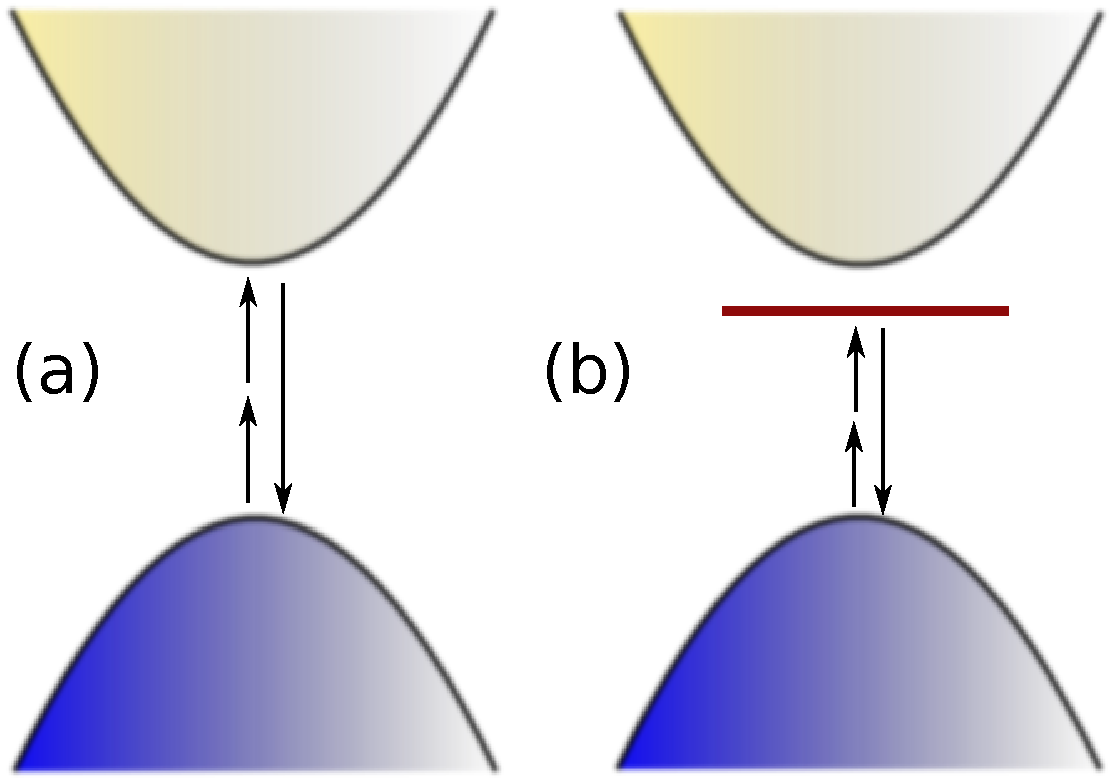
\includegraphics[width=0.4\textwidth]{Figures/exciton}
%\caption{\footnotesize{Schematic representation of  (a) the SHG within the IPA, or (b) accounting for electron-hole interaction. In (a) SHG is given simply by transitions between the valence (blue) and conduction (yellow) manifolds; in (b) electron-hole may lead to the formation of a bound exciton, an atomic-like level (dark red) into the fundamental band gap that strongly modifies the SHG. \label{schemeshg}}}  
%\end{center}
%\end{wrapfigure}   

\begin{figure}[H]
%\begin{wrapfigure}{r}{0.5\textwidth}
    \centering
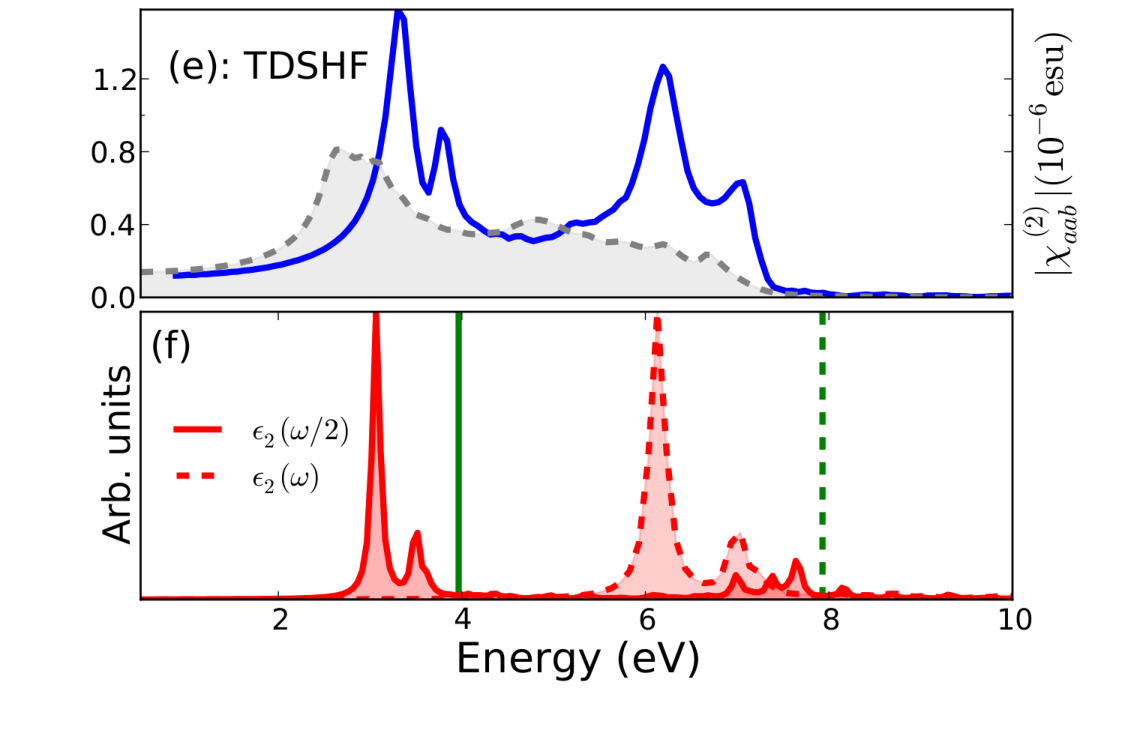
\includegraphics[width=0.5\textwidth]{Figures/eps_and_X2_short}
\caption{\footnotesize{SHG spectra for the h-BN monolayer at different levels of theory [Eq.~\eqref{mbhamiltonian}]: (a) IPA (dashed grey line) and TD-BSE (continous blue line). The imaginary part of the dielectric constant at both $\omega/2$ (red continuous line) and $\omega$ (red dashed line) is reported in (b) at the  TD-BSE level. The vertical lines represent the $GW$ fundamental gap (green dashed line) and half of the $GW$ fundamental gap (green continuous line). \label{absX2bn} [Figure from Ref.\cite{PhysRevB.89.081102}]}}
\end{figure}
%\end{wrapfigure}
Here we present some result performed with the computation scheme presented in previous sections.
At the beginning our computational approach has been validated by direct comparison with calculation in frequencies domain. For example in Fig. ~\ref{fg:SiCQPRPA} we compared our calculations of SHG in SiC and AlAs against the results from Refs.~\cite{PhysRevB.82.235201,PSSB.427.1984}. We found a perfect agreement for SHG in different approximation IPA, QP, TD-Hartree.  Similar comparison has been performed also for third harmonic generation versus simple models and experimental results, see Ref.~\ref{nloptics2013}.\\
Using the methodology developed in the previous section the SHG in many two-materials from h-BN and MoS$_2$, SiC etc. has been studied.\cite{attaccalite2015strong,wei2019second,beach2020strain,mishra2020exciton,attaccalite2019second} The optical absorption of two-dimensional crystals is dominated strongly bound excitons. They offect a perfect test-case for the study of excitonic effects in the non-linear response.
Here we present the simple case of h-BN.
Hexagonal Boron-Nitride is a transparent insulating material with a large band gap of about $6~eV$. Its optical properties are dominated by strong bound excitons and they are nearly independent from the layers arrangement.\cite{PhysRevLett.96.126104,PhysRevLett.100.189701} The single layer h-BN inherits all these properties from its bulk counterpart.
In Fig.~\ref{absX2bn} we report the calculated absolute value of $\chi^{(2)}_{aab} (\omega)$ at different levels of approximation. $\chi^{(2)}_{aab} (\omega)$, where $a$ and $b$ are the in-plane Cartesian directions, is the only independent in-plane component of $\chi^{(2)} (\omega)$: all other components can be obtained from the $\chi^{(2)}_{aab} (\omega)$ with simple symmetry considerations, for instance $\chi^{(2)}_{bbb} (\omega)=-\chi^{(2)}_{aab} (\omega)$. 
At IPA level [Fig.~\ref{absX2bn}(a)], the SHG presents a peak at $2.3~eV$ and a broad structure between $4 - 7 eV$. By comparison with the imaginary part of the dielectric constant $\epsilon_2$ both at $\omega/2$ and  $\omega$ [Fig.~\ref{absX2bn}(b)] calculated at the same level of theory, we can attribute the peak at $2.3~eV$ to two-photon resonances with $\pi \to \pi^*$ transitions, and the broad structure mostly to one-photon resonances with $\pi \to \pi^*$ transitions, with contributions around $7 eV$ of two-photon resonances with $\sigma \to \sigma^*$ transitions.
This level of theory is the one usually employed in theoretical calculations of SHG: in fact results for the h-BN monolayer were previously obtained by Guo and Lin:~\cite{guo2005second} Fig.~\ref{X2bn} shows a very good agreement between our results and those obtained in Ref.~\cite{guo2005second}. In the following we show how effects beyond the IPA---that is the additional terms in Eq.~\eqref{mbhamiltonian}---modify the SHG spectrum.        
We start by adding crystal local field effects, included at the TDH level [Fig.~\ref{absX2bn}(a)]. Because of the weak in-plane inhomogeneity of the h-BN, local field effects are quite small---though they are not negligible as for the absorption spectrum  [Fig.~\ref{absX2bn}(b)]---and results in the reduction of about 20\% of the peak at $2.3~eV$. Next we consider the renormalization of the band structure by quasiparticle corrections within the $GW$ approximation (IPA+$GW$) [Fig.~\ref{absX2bn}(c)]. For h-BN this renormalization can be safely approximated by a rigid shift of the conduction bands. Differently from the absorption spectrum [Fig.~\ref{absX2bn}(d)], the SHG is not simply shifted by $GW$ corrections, but its shape changes remarkably as a consequence of the more involved poles structure of the second order susceptibility.~\cite{PhysRevB.82.235201,hughes1996calculation}
In fact, the IPA+$GW$ shows two peaks: the first at about $4~eV$ is the shifted two-photon $\pi \to \pi^*$  resonances peak which is attenuated by 40\% with respect to IPA  [Fig.~\ref{absX2bn} (a)]; the second very pronounced peak at about $8~eV$ comes from the interference of  $\pi \to \pi^*$  one-photon resonances and  $\sigma \to \sigma^*$ two-photon resonances.  
Finally, in Fig.~\ref{absX2bn}(e) we consider the full Hamiltonian in Eq.~\eqref{mbhamiltonian}. In particular we add the self-energy terms that introduces an attractive interaction between the excited electrons and holes\cite{strinati}. The SHG spectrum presents four sharp and strong peaks and its onset is red-shifted by about $1~eV$ with respect to the the IPA+$GW$ [Fig.~\ref{absX2bn} (c)]. By comparing with the imaginary part of the dielectric constant $\epsilon_2$ both at $\omega/2$ and  $\omega$ [Fig.~\ref{absX2bn} (f)] calculated at the same level of theory, the two couples of peaks can be identified respectively as the two- and one-photon resonances with the excitons at $6$ and $7~eV$.  Fig.~\ref{absX2bn}(e) also shows again the SHG within the IPA to emphasise the striking difference between the two spectra: the TD-BSE spectrum presents features that are missing in IPA and more importantly is twice as strong than IPA at the exciton resonances. 
Excitonic effects in SHG spectrum have been treated as well in a TD-DFT framework\cite{PhysRevB.82.235201} by using the so-called long-range-corrected (LRC) approximation,\cite{LRC} a semi-empirical simple model for the screened electron-hole attraction, that includes only the long-range part of the interaction. In Fig.~\ref{absX2bn}(f) we see the $\epsilon_2$ calculated within the LRC approximation: as earlier recognised, this approximation fails for strong excitons. In fact by tuning the empirical parameter for the screening we could get the position of the first exciton, though its intensity is strongly overestimated (see caption of Fig.~\ref{absX2bn}), but in no way we could get the second excitonic peak. Those pitfalls would be reflected in the SHG spectrum, though we did not test it in our approach. Then clearly the h-BN monolayer and similar low dimensional materials with strong excitonic effects cannot be treated within the approach proposed in Ref.~\cite{PhysRevB.82.235201}.

\section{Conclusions}\label{conclusion}                                        
In this chapter we presented an \ai real-time approach to calculate nonlinear optical properties of extended systems in the length gauge. The key strengths of the proposed approach are first, the correct treatment of the coupling between electrons and the external field and second the possibility to include easily correlation effects beyond the IPA.

Regarding the treatment of the electron-field coupling, following the work of Souza et al.\cite{souza_prb}, we started from the Berry's phase formulation for the dynamical polarisation---a definition consistent with the periodic boundart conditions (PBC)---to derive a covariant numerical expression for the dipole operator in the EOMs.

Note that we worked in the length-gauge even if the velocity gauge may appear a more natural choice. In fact, as opposed to the position operator the velocity operator is consistent with the PBC. However, in the velocity gauge even if the position operator disappears from the Hamiltonian, it reappears in the phase factor for the wave-function~\cite{PhysRevA.36.2763}, so that the problem of re-defining the position operator remains. 
Furthermore, the velocity gauge is plagued by unphysical numerical divergences for the response at low frequencies~\cite{PhysRevB.52.14636}. 
Concerning effects beyond the independent-particle approximation, they are included by simply adding the corresponding single-particle operator to the Hamiltonian. This is an easy task when compared with deriving the corresponding expressions for the nonlinear optical susceptibility.~\cite{PhysRevB.80.155205,PhysRevB.80.165318} As an example, in the present chapter we have included quasi-particle corrections to the band-gap by adding to the Hamiltonian a scissor operator and crystal local-field effects by adding the time-evolution of the Hartree potential. In principle, one can add as well excitonic effects by adding the time-evolution of the screened exchange self-energy (see chapter~\ref{chaptercorr}); or perform a real-time TD-DFT calculations by adding the time-evolution of the exchange-correlation potential (see chapter~\ref{chaptertddft}). Being the focus of this chapter the validation of the proposed approach for calculating nonlinear properties, the inclusion of these correlation effects is discussed in the rest of this work.
We have proved the validity of our approach by comparing our results, obtained from real-time simulations, with results in the literature obtained from direct evaluation of the second order susceptibility in frequency-domain.  

